\documentclass[tikz,border=2pt]{standalone}
\usetikzlibrary{arrows.meta,patterns}
\tikzset{sym/.style={line width=2pt, draw=black, line cap=round, line join=round},
  pw/.style={circle, draw=black, line width=1.2pt, fill=white, minimum size=4.2mm, inner sep=0pt},
  pd/.style={circle, draw=black, line width=1.2pt, fill=black!80, minimum size=4.2mm, inner sep=0pt}}
\newcommand{\beaker}{\draw[sym] (-0.15,2.7) -- (0,2.55) -- (0,0) -- (2.6,0) -- (2.6,2.6);}
\begin{document}
% 16 Pure substances: one kind of particle
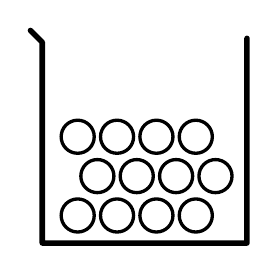
\begin{tikzpicture}\beaker
  \foreach \x/\y in {0.45/0.35,0.95/0.35,1.45/0.35,1.95/0.35,0.7/0.85,1.2/0.85,1.7/0.85,2.2/0.85,0.45/1.35,0.95/1.35,1.45/1.35,1.95/1.35}{\node[pw] at (\x,\y) {};}
\end{tikzpicture}
% 17 Mixtures: two kinds of particle
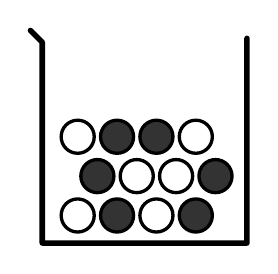
\begin{tikzpicture}\beaker
  \foreach \p/\k in {0.45/0.35/pw,0.95/0.35/pd,1.45/0.35/pw,1.95/0.35/pd,0.7/0.85/pd,1.2/0.85/pw,1.7/0.85/pw,2.2/0.85/pd,0.45/1.35/pw,0.95/1.35/pd,1.45/1.35/pd,1.95/1.35/pw}{}
  \foreach \x/\y/\k in {0.45/0.35/pw,0.95/0.35/pd,1.45/0.35/pw,1.95/0.35/pd,0.7/0.85/pd,1.2/0.85/pw,1.7/0.85/pw,2.2/0.85/pd,0.45/1.35/pw,0.95/1.35/pd,1.45/1.35/pd,1.95/1.35/pw}{\node[\k] at (\x,\y) {};}
\end{tikzpicture}
% 18 Classifying: a flowchart decision
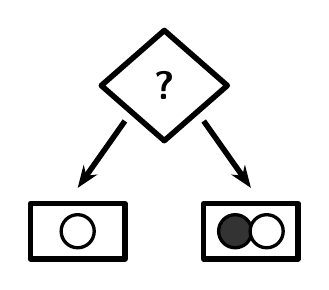
\begin{tikzpicture}
  \draw[sym, fill=white] (1.4,2.9) -- (2.2,2.2) -- (1.4,1.5) -- (0.6,2.2) -- cycle;
  \node[font=\Large\bfseries\sffamily] at (1.4,2.2) {?};
  \draw[black, line width=2pt, -{Stealth[length=8pt]}] (0.9,1.75) -- (0.3,0.9);
  \draw[black, line width=2pt, -{Stealth[length=8pt]}] (1.9,1.75) -- (2.5,0.9);
  \draw[sym] (-0.3,0) rectangle (0.9,0.7); \draw[sym] (1.9,0) rectangle (3.1,0.7);
  \node[pw] at (0.3,0.35) {}; \node[pd] at (2.3,0.35) {}; \node[pw] at (2.7,0.35) {};
\end{tikzpicture}
% 19 Solute, solvent, solution: a sugar cube dissolving
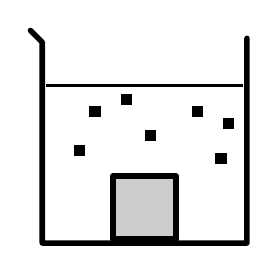
\begin{tikzpicture}\beaker
  \draw[black, line width=1pt] (0.05,2.0) -- (2.55,2.0);
  \draw[sym, fill=black!20] (0.9,0.05) rectangle (1.7,0.85);
  \foreach \x/\y in {0.4/1.1,0.6/1.6,1.3/1.3,1.9/1.6,2.2/1.0,1.0/1.75,2.3/1.45}{\fill (\x,\y) rectangle (\x+0.14,\y+0.14);}
\end{tikzpicture}
% 20 Saturation: solid left undissolved at the bottom
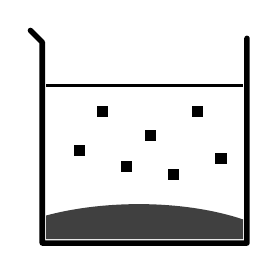
\begin{tikzpicture}\beaker
  \draw[black, line width=1pt] (0.05,2.0) -- (2.55,2.0);
  \fill[black!75] (0.05,0.05) -- (0.05,0.35) .. controls (0.8,0.55) and (1.8,0.55) .. (2.55,0.3) -- (2.55,0.05) -- cycle;
  \foreach \x/\y in {0.4/1.1,0.7/1.6,1.3/1.3,1.9/1.6,2.2/1.0,1.0/0.9,1.6/0.8}{\fill (\x,\y) rectangle (\x+0.14,\y+0.14);}
\end{tikzpicture}
% 21 Solubility curves
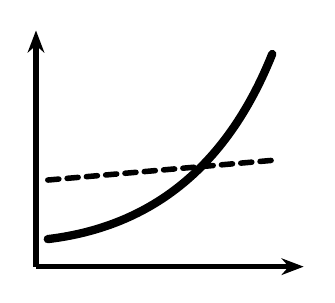
\begin{tikzpicture}
  \draw[black, line width=2pt, -{Stealth[length=8pt]}] (0,0) -- (3.4,0);
  \draw[black, line width=2pt, -{Stealth[length=8pt]}] (0,0) -- (0,3.0);
  \draw[black, line width=3pt, line cap=round] (0.15,0.35) .. controls (1.4,0.5) and (2.4,1.2) .. (3.0,2.7);
  \draw[black, line width=2pt, line cap=round, dash pattern=on 4pt off 3pt] (0.15,1.1) -- (3.0,1.35);
\end{tikzpicture}
% 25 Filtration: funnel, filter paper, flask
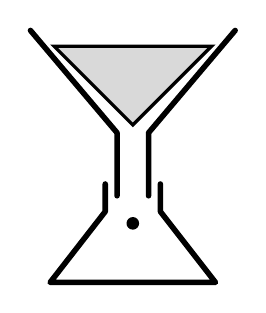
\begin{tikzpicture}
  \draw[sym] (0,3.2) -- (1.1,1.9) -- (1.1,1.1) (2.6,3.2) -- (1.5,1.9) -- (1.5,1.1);
  \draw[black, line width=1.2pt, fill=black!15] (0.3,3.0) -- (1.3,2.0) -- (2.3,3.0) -- cycle;
  \draw[sym] (0.95,1.25) -- (0.95,0.9) -- (0.25,0) -- (2.35,0) -- (1.65,0.9) -- (1.65,1.25);
  \fill (1.3,0.75) circle (0.08);
\end{tikzpicture}
% 26 Evaporation and crystallisation: basin over a flame, crystals
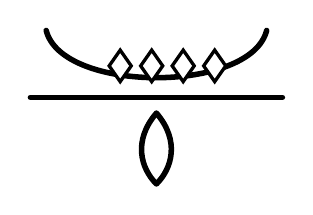
\begin{tikzpicture}
  \draw[sym] (0,2.0) .. controls (0.2,1.2) and (2.6,1.2) .. (2.8,2.0);
  \foreach \x in {0.8,1.2,1.6,2.0}{\draw[black, line width=1.2pt, fill=white] (\x,1.55) -- (\x+0.14,1.75) -- (\x+0.28,1.55) -- (\x+0.14,1.35) -- cycle;}
  \draw[sym] (-0.2,1.15) -- (3.0,1.15);
  \draw[sym, fill=white] (1.4,0.95) .. controls (1.1,0.6) and (1.2,0.25) .. (1.4,0.05) .. controls (1.6,0.25) and (1.7,0.6) .. (1.4,0.95);
\end{tikzpicture}
% 27 Chromatography: a paper strip with spots separated
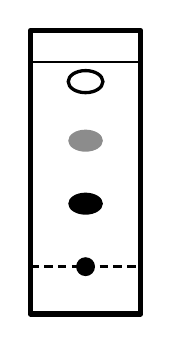
\begin{tikzpicture}
  \draw[sym] (0.6,0) rectangle (2.0,3.6);
  \draw[black, line width=1pt, dash pattern=on 3pt off 2pt] (0.6,0.6) -- (2.0,0.6);
  \fill (1.3,0.6) circle (0.12);
  \fill[black] (1.3,1.4) ellipse (0.22 and 0.14);
  \fill[black!45] (1.3,2.2) ellipse (0.22 and 0.14);
  \draw[black, line width=1.2pt] (1.3,2.95) ellipse (0.22 and 0.14);
  \draw[black, line width=1pt] (0.6,3.2) -- (2.0,3.2);
\end{tikzpicture}
\end{document}
